\documentclass[12pt]{article}

\usepackage[top=0.75in,bottom=0.75in,left=0.5in,right=0.75in]{geometry}
\usepackage{amsmath,amssymb,multirow,graphicx,wrapfig}

\newcommand{\bx}{\mathbf{x}}
\newcommand{\by}{\mathbf{y}}
\newcommand{\bn}{\mathbf{n}}
\newcommand{\bu}{\mathbf{u}}
\newcommand{\bv}{\mathbf{v}}
\newcommand{\bd}{\mathbf{d}}
\newcommand{\ff}{\mathbf{f}}
\newcommand{\bF}{\mathbf{F}}
\newcommand{\bU}{\mathbf{U}}
\newcommand{\phie}{\phi_{\epsilon}}
\newcommand{\psie}{\psi_{\epsilon}}
\newcommand{\vphie}{\varphi_{\epsilon}}
\newcommand{\eps}{\epsilon}

\newcommand{\bee}[1]{\begin{equation} #1 \end{equation}}
\newcommand{\baa}[1]{\begin{align} #1 \end{align}}
\newcommand{\bees}[1]{\begin{equation*} #1 \end{equation*}}
\newcommand{\baas}[1]{\begin{align*} #1 \end{align*}}


\newcommand{\dd}[2]{\ensuremath{\frac{\text{d} #1}{\text{d} #2}}}
\newcommand{\ddd}[2]{\ensuremath{\frac{\text{d}^2 #1}{\text{d} {#2}^2}}}
\newcommand{\pd}[2]{\ensuremath{\frac{\partial #1}{\partial #2}}}
\newcommand{\pdd}[2]{\ensuremath{\frac{\partial^2 #1}{\partial {#2}^2}}}
\newcommand{\pddd}[3]{\ensuremath{\frac{\partial^2 #1}{\partial #2 \partial #3}}}
\newcommand{\minus}[2]{\ensuremath{#1 \text{-} #2}}

\title{Resolving nearly singular integrals in regularized Stokeslets using a linear boundary element method with exact integration}
\author{Bree Cummins, Ricardo Cortez, Mike Nicholas}

\renewcommand{\abstractname}{Summary}

\begin{document}
	
	\maketitle
	
	\begin{abstract}Fundamental solutions to the Stokes equations (Stokeslets) exhibit singular behavior at forcing locations, and nearly singular behavior close to these locations. For forces along a curve in two dimensions or spread across a surface in three dimensions, the singularities are integrable, although the integration has to be handled carefully. However, for points in 2D, or curves and points in 3D, the singularities are not integrable. The method of regularized Stokeslets (Cortez 2001) transforms the singular Stokeslet behavior into nearly singular behavior at the force points. This reduces the problem of singular integration to nearly singular integration, and also admits finite solutions for clusters of isolated points and slender bodies in three dimensions. 
	
	The method of regularized Stokeslets was originally formulated in terms of a Riemann sum approximation to the boundary integral equation over curves and surfaces. Because the regularized kernel is nearly singular, one can always find points close enough to the boundary where the peak in the integration kernel is too sharp to be captured. One solution is to cluster integration points near the approach of a point of interest to the boundary (Gaussian quadrature or change of coordinates). Another solution is to exactly integrate the kernel, although this cannot be done in all cases. Smith (2010) pointed out that a linear boundary element (BE) method can be used to approximate the boundary integral along a curve, and that this method admits exact integration for a known regularized kernel.
	
	The purpose of this paper is to apply a linear BE aproximation to the boundary integral equation that allows exact integration of regularized Stokeslet kernels along curves embedded in two and three dimensional space. Different regularizations will be presented and test cases for numerically verifying the method will be discussed.
\end{abstract}
	
	\section{BE formulation of regularized Stokeslets}

	The solution to the regularized Stokes equations in 2D or 3D with forcing over a curve is:
	%%%%%%%%%%%%%%%%%%%%%%%%%%%
	\begin{eqnarray}\label{usoln}
		\bu(\bx_*) &=& \frac{1}{\mu} \int_{C} H_1(r)\ff(\bx) + H_2(r)[\ff(\bx) \cdot (\bx_* - \bx)](\bx_* - \bx) \,d\ell(\bx),
	\end{eqnarray}
	%%%%%%%%%%%%%%%%%%%%%%%%%%%%
	where $\bx = (x,y)$ or $ (x,y,z)$ depending on dimension, $\bx_*$ is the point where we want to know the velocity $\bu = (u,v)$ or $(u,v,w)$, the boundary curve is $C$, and the vector-valued function $\ff$ is the applied forcing along $C$.  The variable $r$ is distance from the point of interest, $r= || \bx_* - \bx ||$, and the specific forms of $H_1(r)$ and $H_2(r)$ depend on the particular blob function chosen for the regularization. Examples of $H_1(r)$ and $H_2(r)$ will be given later on. 
	
	We employ a boundary element method to approximate the line integral in Eq.~\eqref{usoln}. We discretize $\partial \Omega$ into linear chords and use linear interpolation to approximate the forcing function $\ff$ on each chord. As will be seen later, this allows us to derive closed form expressions for the moments of $H_1$ and $H_2$. 
	
		%%%%%%%%%%%%%%%%%%%%%%%%%%%%%%%%%%%%%%%%%%%%%%%%%%%%%%
		 \begin{wrapfigure}{l}{0.39\textwidth}
			\vspace{-3mm} 
			\fbox{
			    \begin{minipage}[t][0.26\textheight]{0.36\textwidth}
				\begin{center}
					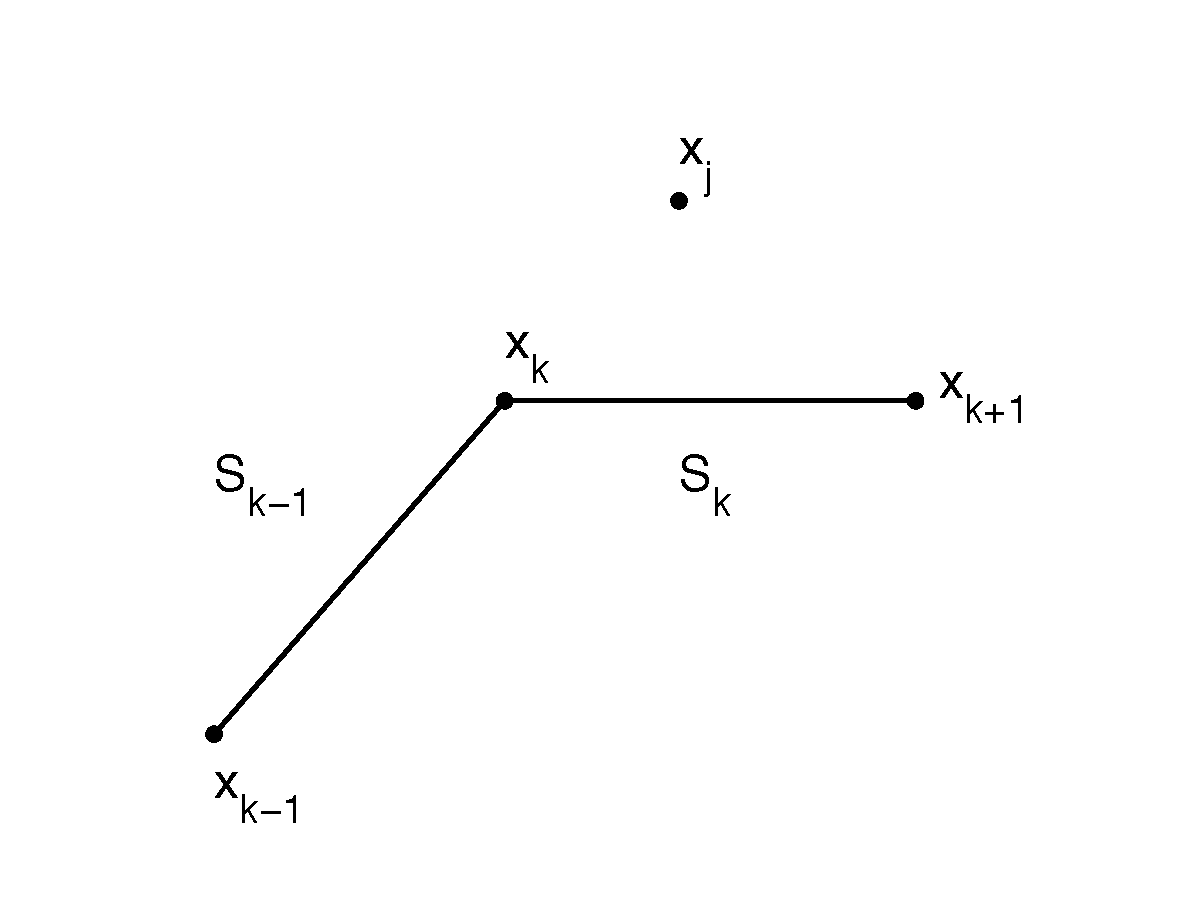
\includegraphics[width=0.96\textwidth]{ijonly.pdf} 
					\vspace{-2mm} 
					\caption{\small{Two boundary chords $S_{k-1}$, $S_k$ in relation to an arbitrary point $x_j$.}}
				\end{center}
					\label{ijonly}
			    \end{minipage}
			  }
				\vspace{-5mm}
		\end{wrapfigure}
	%%%%%%%%%%%%%%%%%%%%%%%%%%%%%%%%%%%%%%%%%%%%%%%%%%%%%%
	We consider the effect of one force, $\ff_k := \ff(\bx_k)$, on the velocity $\bu$ at an arbitrary point $\bx_j$. The force is located at the join of two boundary chords  (see Fig.~\ref{ijonly}). We parameterize the equations of the chords:
	%%%%%%%%%%%%%%%%%%%%%%%%%%%%%%%%%%%%%%%%%%%%%%%%%%%%%%
	\baas{
	S_{k-1}: & \qquad \bx(s) = (1-s)\bx_{k-1} 	+ s\bx_k \\
	S_k: &  \qquad \bx(z) = (1-z)\bx_k 		+ z\bx_{k+1}, 
	} 
	%%%%%%%%%%%%%%%%%%%%%%%%%%%%%%%%%%%%%%%%%%%%%%%%%%%%
	where both $s$ and $z$ vary from 0 to 1.
	The linear interpolations for the forces along the chords are:
	%%%%%%%%%%%%%%%%%%%%%%%%%%%%%%%%%%%%%%%%%%%%%%%%%%%%%%
	\baas{
	S_{k-1}: & \qquad \ff(s) = (1-s)\ff_{k-1} 	+ s\ff_k \\
	S_k: &  \qquad \ff(z) = (1-z)\ff_k 		+ z\ff_{k+1},
	} 
	%%%%%%%%%%%%%%%%%%%%%%%%%%%%%%%%%%%%%%%%%%%%%%%%%%%%
	If $\ff_{k-1} = 0 = \ff_{k+1}$ and $\partial\Omega = S_{k-1} \cup S_k$, the velocity $\bu_j := \bu(\bx_j)$ from Eq.~\eqref{usoln} becomes
	%%%%%%%%%%%%%%%%%%%%%%%%%%%%%%%%%%%%%%%%%%%%%%%%%%%%
	\baa{
	\bu_j &= \frac{1}{\mu} \int_0^1 \left[sH_1(r)\ff_k + sH_2(r)[\ff_k \cdot (\bx_j - \bx(s))](\bx_j - \bx(s))\right]\, h_{k-1} \,ds \nonumber \\
	&+ \frac{1}{\mu} \int_0^1 \left[(1-z)H_1(r)\ff_k + (1-z)H_2(r)[\ff_k \cdot (\bx_j - \bx(z))](\bx_j - \bx(z))\right]\, h_{k+1} \,dz, \label{ujk}
	}
	%%%%%%%%%%%%%%%%%%%%%%%%%%%%%%%%%%%%%%%%%%%%%%%%%%%%
	where $r(s) =|| \bx_j - \bx(s) ||$ in the first integral, $r(z) = || \bx_j - \bx(z) ||$ in the second, and $h$ is the arc length due to the change of variables: $h_{k-1} = || d\bx(s)/ds || = || \bx_k - \bx_{k-1}||$ and $h_{k+1} = || d\bx(z)/dz || = || \bx_{k+1} - \bx_{k}||$. 
	
	We perform a coordinate change to reduce the number of terms in Eq.~\eqref{ujk}. If we make the substitution $z = 1-s$, then the equations $\bx_j - \bx$ along the chords look the same except that one uses $\bx_{k-1}$ and the other uses $\bx_{k+1}$:
	%%%%%%%%%%%%%%%%%%%%%%%%%%%%%%%%%%%%%%%%%%%%%%%%%%%%
	\baas{
	S_{k-1}: & \qquad  \bx_j - \bx(s) \qquad = \bx_j - \bx_{k-1} + s(\bx_{k-1} - \bx_k) \\
	S_{k}: & \qquad  \bx_j - \bx(1-s) \, = \bx_j - \bx_{k+1} + s(\bx_{k+1} - \bx_k). \nonumber
	}
	%%%%%%%%%%%%%%%%%%%%%%%%%%%%%%%%%%%%%%%%%%%%%%%%%%%%
	We write the arguments of $H_1$ and $H_2$ as 
	%%%%%%%%%%%%%%%%%%%%%%%%%%%%%%%%%%%%%%%%%%%%%%%%%%%%
	\baa{
	r_{k\pm 1}(s) & = || \bx_j - \bx_{k\pm 1} + s(\bx_{k\pm 1} - \bx_k)|| ,  \label{rk-1} 
	}
	%%%%%%%%%%%%%%%%%%%%%%%%%%%%%%%%%%%%%%%%%%%%%%%%%%%%
		with $\bx_{k-1}$ over the first chord and $\bx_{k+1}$ over the second. Since the coordinate change $z=1-s$ implies $\int_0^1 ds  = \int_0^1 dz$ and the arc length $h_{k+1}$ is unchanged, we rewrite Eq.~\eqref{ujk} as
	%%%%%%%%%%%%%%%%%%%%%%%%%%%%%%%%%%%%%%%%%%%%%%%%%%%%
	\baa{
	\bu_j &= \frac{h_{k-1}}{\mu} \int_0^1 sH_1(r_{k-1})\ff_k + sH_2(r_{k-1})[\ff_k \cdot (\bx_j - \bx(s))](\bx_j - \bx(s)) \,ds \nonumber \\
	&+ \frac{h_{k+1}}{\mu} \int_0^1 sH_1(r_{k+1})\ff_k + sH_2(r_{k+1})[\ff_k \cdot (\bx_j - \bx(1-s))](\bx_j - \bx(1-s)) \,ds \nonumber \\
	& =: \bU_{k-1} + \bU_{k+1}, \label{ujkcc}
	}
	%%%%%%%%%%%%%%%%%%%%%%%%%%%%%%%%%%%%%%%%%%%%%%%%%%%%
	where the last line introduces convenient notation.
	 	
 	The vector $[\ff_k \cdot (\bx_j - \bx(s))](\bx_j - \bx(s))$ may be written as a matrix multiplication $\mathcal{M}_{k-1}(s)\ff_k$, where 
	%%%%%%%%%%%%%%%%%%%%%%%%%%%%%%%%%%%%%%%%%%%%%%%%%%%%
	\baas{
	\mathcal{M}_{k-1}(s)  & = (\bx_j - \bx(s))(\bx_j - \bx(s))^T
	} 
	%%%%%%%%%%%%%%%%%%%%%%%%%%%%%%%%%%%%%%%%%%%%%%%%%%%%
	with superscript $T$ denoting transpose. Since $\mathcal{M}_{k-1}(s)$ is the square of a linear function, it can be rewritten as a quadratic with matrices of coefficients (see Appendix~\ref{app:matentries}):
	%%%%%%%%%%%%%%%%%%%%%%%%%%%%%%%%%%%%%%%%%%%%%%%%%%%%
	\baas{
	\mathcal{M}_{k-1}(s)  & \equiv \mathcal{A}_{k-1}s^2 + \mathcal{B}_{k-1}s + \mathcal{C}_{k-1}.
	} 
	%%%%%%%%%%%%%%%%%%%%%%%%%%%%%%%%%%%%%%%%%%%%%%%%%%%%
	We rewrite the first velocity term as
	%%%%%%%%%%%%%%%%%%%%%%%%%%%%%%%%%%%%%%%%%%%%%%%%%%%%
	\baa{
	\frac{\mu}{h_{k-1}}\bU_{k-1} & = \ff_k \int_0^1 sH_1(r) \,ds + \mathcal{A}_{k-1} \ff_k \int_0^1 s^3 H_2(r) \, ds + \mathcal{B}_{k-1} \ff_k \int_0^1 s^2 H_2(r) \, ds + \mathcal{C}_{k-1} \ff_k \int_0^1 s H_2(r)\,ds \nonumber \\
	& = \left[ \mathcal{I}\int_0^1 sH_1(r) \,ds + \mathcal{A}_{k-1}\int_0^1 s^3 H_2(r) \, ds + \mathcal{B}_{k-1} \int_0^1 s^2 H_2(r) \, ds + \mathcal{C}_{k-1} \int_0^1 s H_2(r)\,ds \right]  \ff_k  \nonumber \\
	\Rightarrow \bU_{k-1} & \equiv \frac{h_{k-1}}{\mu}\mathcal{K}_{k-1} \ff_k, \label{contrib1}
	}
	%%%%%%%%%%%%%%%%%%%%%%%%%%%%%%%%%%%%%%%%%%%%%%%%%%%%
	where $\mathcal{I}$ is the appropriately sized identity matrix, $\mathcal{K}_{k-1}$ is a kernel relating force to velocity, and $r \equiv r_{k-1}(s)$. Similarly, 
	%%%%%%%%%%%%%%%%%%%%%%%%%%%%%%%%%%%%%%%%%%%%%%%%%%%%
	\baa{
	\frac{\mu}{h_{k+1}}\bU_{k+1} & = \left[ \mathcal{I}\int_0^1 sH_1(r) \,ds + \mathcal{A}_{k+1}\int_0^1 s^3 H_2(r) \, ds + \mathcal{B}_{k+1} \int_0^1 s^2 H_2(r) \, ds + \mathcal{C}_{k+1} \int_0^1 s H_2(r)\,ds \right]  \ff_k  \nonumber \\
	\Rightarrow \bU_{k+1} & \equiv \frac{h_{k+1}}{\mu}\mathcal{K}_{k+1} \ff_k, \label{contrib2}
	}
	%%%%%%%%%%%%%%%%%%%%%%%%%%%%%%%%%%%%%%%%%%%%%%%%%%%%
	where $r \equiv r_{k+1}(s)$. We finally have from Eq.~\eqref{ujkcc} and the above work:
	%%%%%%%%%%%%%%%%%%%%%%%%%%%%%%%%%%%%%%%%%%%%%%%%%%%%
	\baa{
	\bu_j & = \frac{h_{k-1}}{\mu}\mathcal{K}_{k-1} \ff_k + \frac{h_{k+1}}{\mu}\mathcal{K}_{k+1} \ff_k, \label{ujkmat}
	}
	%%%%%%%%%%%%%%%%%%%%%%%%%%%%%%%%%%%%%%%%%%%%%%%%%%%%
	
	The advantage of this formulation is that all the constant factors have been pulled out from the integrals, leaving only the moments of $H_1$ and $H_2$ to be calculated for specific blob functions. The moments are then used to construct the kernels $\mathcal{K}_{k-1}$ and $\mathcal{K}_{k+1}$.
	
	
	\section{Generalizations to multiple force points}
	
	Equation~\eqref{ujkmat} is easily generalized to an open curve discretized into $N$ chords with endpoints $\bx_0, \bx_1, \dotsc, \bx_N$:
	%%%%%%%%%%%%%%%%%%%%%%%%%%%%%%%%%%
	\baa{
	\bu_j^{\text{open}} & = \frac{h_{k-1}}{\mu}\sum_{k=1}^N \mathcal{K}_{k-1}\ff_k + \frac{h_{k+1}}{\mu}\sum_{k=0}^{N-1} \mathcal{K}_{k+1}\ff_k \nonumber \\
	& =  \frac{1}{\mu}\left[  h_1\mathcal{K}_{1}\ff_0 + h_{N-1}\mathcal{K}_{N-1}\ff_N  + \sum_{k=1}^{N-1} \left(h_{k-1}\mathcal{K}_{k-1}+h_{k+1}\mathcal{K}_{k+1}\right) \ff_k  \right]\label{opencurve}
	}	
	%%%%%%%%%%%%%%%%%%%%%%%%%%%%%%%%%%
	For a closed curve with $N+1$ chords, we have circular indexing: 
	%%%%%%%%%%%%%%%%%%%%%%%%%%%%%%%%%%
	\baa{
	\bu_j^{\text{closed}} & = \frac{h_{k-1}}{\mu}\sum_{k=0}^N \mathcal{K}_{k-1}\ff_k + \frac{h_{k+1}}{\mu}\sum_{k=0}^{N} \mathcal{K}_{k+1}\ff_k \nonumber \\
	& =  \frac{1}{\mu}\left[  h_N\mathcal{K}_{N}\ff_0 + h_1\mathcal{K}_{1}\ff_0+ h_{N-1}\mathcal{K}_{N-1}\ff_N + h_0\mathcal{K}_{0}\ff_N + \sum_{k=1}^{N-1} \left(h_{k-1}\mathcal{K}_{k-1}+h_{k+1}\mathcal{K}_{k+1}\right) \ff_k  \right] \nonumber \\
	& = \frac{1}{\mu}\left[  h_N\mathcal{K}_{N}\ff_0 + h_0\mathcal{K}_{0}\ff_N \right] + \bu_j^{\text{open}}. \label{closedcurve}
	}	
	%%%%%%%%%%%%%%%%%%%%%%%%%%%%%%%%%%
	 
	
	There are times when the forcing function $\ff(\bx)$ is not known along $\partial\Omega$; instead, boundary conditions are given in terms of velocity. For Dirichlet boundary conditions, 
	%%%%%%%%%%%%%%%%%%%%%%%%%%%%%%%%%%
	\[ \bu\big|_{\partial\Omega} = \bv(\bx),\]
	%%%%%%%%%%%%%%%%%%%%%%%%%%%%%%%%%%
	one can solve the linear system
	%%%%%%%%%%%%%%%%%%%%%%%%%%%%%%%%%%
	\baa{
	\bv_0 & =  \frac{1}{\mu}\sum_{k=1}^N h_{k-1}\mathcal{K}_{k-1}\ff_k +  \frac{1}{\mu}\sum_{k=0}^{N-1} h_{k+1}\mathcal{K}_{k+1}\ff_k  \nonumber \\
	& \vdots  \nonumber \\
	\bv_N & =  \frac{1}{\mu}\sum_{k=1}^N h_{k-1}\mathcal{K}_{k-1}\ff_k +  \frac{1}{\mu}\sum_{k=0}^{N-1} h_{k+1}\mathcal{K}_{k+1}\ff_k, \label{linsys}
	}
	for the set of $\ff_k$, where $\bx_j$ in each of the kernels is the location of $\bv_j$. The set of $\ff_k$ are then used to find velocities anywhere in the domain.
	%%%%%%%%%%%%%%%%%%%%%%%%%%%%%%%%%%
	
	
	
	\section{2D regularized Stokeslets}
	
	In two dimensions, we use the following blob function with associated $H_1$ and $H_2$:
	%%%%%%%%%%%%%%%%%%%%%%%%%%%%%%%%%%
	\baas{
	\phie(r) = \frac{2\eps^4}{\pi(r^2 + \eps^2)^3}, & \qquad H_1(r) = \frac{1}{4\pi}\left(\frac{\eps^2}{r^2 + \eps^2} - \frac{1}{2}\ln \left( r^2 + \eps^2 \right)\right), &  H_2(r) = \frac{1}{4\pi}\left(\frac{1}{r^2 + \eps^2}\right).
	} 
	%%%%%%%%%%%%%%%%%%%%%%%%%%%%%%%%%%
	In this case, both $H_1$ and $H_2$ are functions of $r^2(s)$, which has the form (see Eq.~\eqref{rk-1})
	%%%%%%%%%%%%%%%%%%%%%%%%%%%%%%%%%%%%%%%%%%%%%%%%%%%%
	\baas{
	r^2_{k\pm 1}(s) & = || \bx_j - \bx_{k\pm 1} ||^2 + 2s(\bx_{k\pm 1} - \bx_k)\cdot(\bx_{k\pm 1} - \bx_k) + s^2 || \bx_{k\pm 1} - \bx_k ||^2,
	}
	%%%%%%%%%%%%%%%%%%%%%%%%%%%%%%%%%%%%%%%%%%%%%%%%%%%%
	with $\bx_{k-1}$ on the first chord and $\bx_{k+1}$ on the second. 
	From this equation, we see that $r^2$ is a quadratic in $s$. Based on the form of $H_1$ and $H_2$, we choose to write $r^2 + \eps^2 = as^2 + bs + c$, with
	%%%%%%%%%%%%%%%%%%%%%%%%%%%%%%%%%%
	\baa{
	a & = || \bx_{k\pm 1} - \bx_k ||^2, & b & =  2(\bx_{k\pm 1} - \bx_k ) \cdot (\bx_j - \bx_{k\pm 1} ), & c & = || \bx_j - \bx_{k\pm 1}||^2 + \eps^2. \label{coeffabc}
	}
	%%%%%%%%%%%%%%%%%%%%%%%%%%%%%%%%%%
	 We define the integrals: 
	%%%%%%%%%%%%%%%%%%%%%%%%%%%%%%%%%%
	\baas{
	I_1 & = \int_0^1 \frac{s}{2}\ln \left( as^2 + bs + c \right) \, ds & I_3 & = \int_0^1 \frac{s^2}{as^2 + bs + c} \, ds \\
	I_2 & = \int_0^1 \frac{s}{as^2 + bs + c} \, ds  & I_4 & = \int_0^1 \frac{s^3}{as^2 + bs + c} \, ds. 
	}
	%%%%%%%%%%%%%%%%%%%%%%%%%%%%%%%%%%
	Then the kernel associated with chord $S_{k-1}$, Eq.~\eqref{contrib1}, may be written
	%%%%%%%%%%%%%%%%%%%%%%%%%%%%%%%%%%
	\baa{
	\mathcal{K}_{k-1} &= \frac{1}{4\pi}\left[\left(\eps^2 I_2 - I_1\right)\mathcal{I} + \mathcal{A} I_4 + \mathcal{B} I_3 + \mathcal{C} I_2\right] \nonumber \\
	& =  \frac{1}{4\pi}\left[- I_1\mathcal{I} + \left(\mathcal{C} + \eps^2\mathcal{I}\right) I_2 + \mathcal{B} I_3 + \mathcal{A} I_4\right], \label{Kk-12D}
	}	
	%%%%%%%%%%%%%%%%%%%%%%%%%%%%%%%%%%
	where $\mathcal{A}$, $\mathcal{B}$, $\mathcal{C}$, $a$, $b$, and $c$ all depend on $\bx_{k-1}$. The kernel from $S_k$, $\mathcal{K}_{k+1}$, is defined analogously by replacing every instance of $\bx_{k-1}$ with $\bx_{k+1}$. 

	We solved the integrals using Mathematica. Let
	%%%%%%%%%%%%%%%%%%%%%%%%%%%%%%%%%%
	\baa{
	D & := b^2 - 4ac, & L(s) & :=  \ln \left( as^2 + bs + c \right), & A(s) & := \arctan\left(\dfrac{b + 2as}{\sqrt{-D}}\right). \nonumber
	}
	%%%%%%%%%%%%%%%%%%%%%%%%%%%%%%%%%%
	Since $r^2 + \eps^2 > 0$, the discriminant is always negative: $D < 0$. This implies that the functions $L(s)$ and $A(s)$ are well-defined $\forall \; s$. Using these definitions,
	\baa{
	I_1 & = \Bigg[\frac{-b\sqrt{-D}}{4a^2}A(s) + \frac{-b^2 + 2ac + 2a^2s^2}{8a^2}L(s) + \frac{s(b-as)}{4a} \Bigg]_{s=0}^{s=1} \nonumber \\
	I_2 & = \Bigg[\frac{-b}{a\sqrt{-D}}A(s) + \frac{1}{2a}L(s) \Bigg]_{s=0}^{s=1} \nonumber \\
	I_3 & = \Bigg[\frac{b^2 - 2ac}{a^2\sqrt{-D}}A(s) - \frac{b}{2a^2}L(s) + \frac{s}{a}\Bigg]_{s=0}^{s=1} \nonumber \\
	I_4 & = \Bigg[\frac{-b(b^2 - 3ac)}{a^3\sqrt{-D}}A(s) + \frac{b^2 - ac}{2a^3}L(s) + \frac{s(-2b +as)}{2a^2} \Bigg]_{s=0}^{s=1}. \label{2Dints}
	}
	

	\section{Singular 2D Stokeslets}
	
	In the case of a curve in 2D, a Stokeslet representation is integrable, and the same linear BEM may be applied. To derive this case, we set $\eps = 0$ in our expressions above. When $\bx_j = \bx_k$, then the integrals $I_1,\dotsc,I_4$ are singular as they are written in Eq.~\eqref{2Dints}, so some rewriting is required in this special case.
	
	For $\bx_j = \bx_k$ and $\eps = 0$, the coefficients $a,b,c$ in Eq.~\eqref{coeffabc} fulfill the relationships $c = a$ and $b = -2a$ for a nonzero chord length $a$. We rewrite $as^2 + bs + c = as^2 -2as + a = a(s-1)^2$, and then examine the integrals $I_1,\dotsc,I_4$ (see Appendix~\ref{singularints} for details):
	%%%%%%%%%%%%%%%%%%%%%%%%%%%%%%%%%%
	\baas{
	I_1 &= \frac{\ln(a) - 3}{4}  & I_3 &= \frac{1}{a} + \frac{2}{a}\int_{-1}^0 \frac{1}{z} \, dz + \frac{1}{a}\int_{-1}^0 \frac{1}{z^2} \, dz \\
	I_2 &= \frac{1}{a}\int_{-1}^0 \frac{1}{z} \, dz + \frac{1}{a}\int_{-1}^0 \frac{1}{z^2} \, dz & I_4 &= \frac{5}{2a} + \frac{3}{a}\int_{-1}^0 \frac{1}{z} \, dz + \frac{1}{a}\int_{-1}^0 \frac{1}{z^2} \, dz.
	}
	%%%%%%%%%%%%%%%%%%%%%%%%%%%%%%%%%%
	
	From Appendix~\ref{app:matentries}, we see that when $\bx_j = \bx_k$, $\mathcal{A},\mathcal{B},\mathcal{C}$ have the same relationships as $a,b,c$: $\mathcal{C} = \mathcal{A}$ and $\mathcal{B} = -2\mathcal{A}$. Using this fact and $\eps = 0$, Eq.~\eqref{Kk-12D} becomes
	%%%%%%%%%%%%%%%%%%%%%%%%%%%%%%%%%%
	\baas{
	\mathcal{K}_{k-1} & =  \frac{1}{4\pi}\left[- I_1\mathcal{I} + \mathcal{A} I_2 - 2\mathcal{A} I_3 + \mathcal{A} I_4\right] \\
	&= \frac{1}{4\pi}\left[\frac{-\ln(a) + 3}{4} \mathcal{I} + \frac{\mathcal{A}}{a}\left(- 2 + \frac{5}{2} + \left( 1 -2  +1 \right) \int_{-1}^0 \frac{1}{z^2} \, dz + (1 -4 +3) \int_{-1}^0 \frac{1}{z} \, dz \right)\right]\\
	& = \frac{1}{4\pi}\left[\frac{-\ln(a) + 3}{4} \mathcal{I} + \frac{1}{2a}\mathcal{A} \right].
	}	
	%%%%%%%%%%%%%%%%%%%%%%%%%%%%%%%%%%
	
	
	
	\section{Test Cases}
	
	\subsection{2D Closed Curve}\label{sec:2Dclosedcurve} 
	\textbf{Problem Statement:} Consider an infinitely long cylinder of radius $a$ translating steadily perpendicular to its long axis in an infinite fluid with viscosity $\mu=1.0$. If we take a horizontal slice of the domain, then we see a steadily translating circle in 2D. With steady velocity $\bu = (1,0)$, the exact solution to this test case for $r>a$ is a combination of a Stokeslet and a dipole at the origin:
	%%%%%%%%%%%%%%%%%%%%%%%%%%%%%%%%%%
	\begin{eqnarray}\label{exactsoln}
		\bu(\bx) &=& \frac{-\ff_0}{8\pi}\left( 2\ln\lvert\bx\rvert - a^2/\lvert \bx \rvert^2 \right) + \frac{\left(\ff_0 \cdot \bx \right)\bx}{4\pi\lvert \bx \rvert^2}\left(1-a^2/\lvert \bx \rvert^2\right) \nonumber \\
		\ff_0 &=& \frac{8\pi}{1-2\ln(a)}\begin{pmatrix} 1 \\ 0 \end{pmatrix}.
	\end{eqnarray}
	%%%%%%%%%%%%%%%%%%%%%%%%%%%%%%%%%%
	\textbf{Q: What happened to the fluid viscosity?}\\ \vspace{0.5mm} \\
	In order to approximate this solution using the linear BEM regularized Stokeslet method, we first solve for the forcing along the boundary as in Eq.~\eqref{linsys} with $\bv = (1,0)$ at all points on the circle. We then use these forces to find the velocity at various points outside the circle. 
	
	As an extra check for code correctness, we provide some matrix entries in reduced form in Appendix~\ref{app:2Dtestcase}.\\ \vspace{0.5mm} \\
	\textbf{Numerical Results:} \\
	\begin{table}[!h]
		\centering
	\begin{tabular}{|c|c|c|c|c|c|c|c|c|}
		\hline
		 & \multicolumn{2}{|c|}{$R=$1.001} & \multicolumn{2}{|c|}{$R=$1.01} & \multicolumn{2}{|c|}{$R=$1.1} & \multicolumn{2}{|c|}{$R=$1.25} \\
		\hline
		$N$ & error & rate & error & rate & error & rate & error & rate \\
		\hline
		  16   &   1.1958e-03 &    &  5.8816e-03  &     & 1.1107e-02  &   &  7.0432e-03 & 	     \\
		  32   &   5.2986e-04 &  1.2 &  2.3242e-03  & 1.3  & 3.1302e-03  & 1.8 &  1.8587e-03 & 	1.9     \\
		  64   &   2.2175e-04 &  1.3 &  8.1996e-04  & 1.5  & 8.0005e-04  & 2.0 &  4.7740e-04 & 	2.0     \\
		 128   &   8.5958e-05 &  1.4 &  2.5016e-04  & 1.7  & 1.9951e-04  & 2.0 &  1.1919e-04 & 	2.0     \\
		 256   &   2.8715e-05 &  1.6 &  6.2480e-05  & 2.0  & 4.6487e-05  & 2.1 &  2.7754e-05 & 	2.1     \\
		 512   &   5.8466e-06 &  2.3 &  1.0376e-05  & 2.6  & 7.7864e-06  & 2.6 &  4.6480e-06 & 	2.6     \\
		\hline
	\end{tabular}
	\caption{$\eps$ = 1.e-5, $x = R\cos(\pi/4)$, $y=R\sin(\pi/4)$.}
\end{table}

	
\section{Calculating exact integrals over curves in 3D}

In three dimensions, we use the following blob function with associated $H_1$ and $H_2$:
\baas{
\vphie(r) &= \frac{15\eps^4}{8\pi(r^2+\eps^2)^{7/2}}, & H_1(r) &= \frac{1}{8\pi}\frac{r^2 + 2\eps^2}{\left( r^2 + \eps^2\right)^{3/2}}, & H_2(r) &= \frac{1}{8\pi}\frac{1}{\left( r^2 + \eps^2\right)^{3/2}}.
}
Again, we may write $r^2 + \eps^2 = as^2 + bs +c$ using the same definitions as in Eq.~\eqref{coeffabc}, noting that $\bx$ is now three dimensional. If we then define 	%%%%%%%%%%%%%%%%%%%%%%%%%%%%%%%%
\baas{
	I_{1} &= \int_0^1   \frac{s}{\left(as^2 + bs +c\right)^{3/2}}\,\text{ds}, & I_{2} &= \int_0^1 \frac{s^2}{\left(as^2 + bs +c\right)^{3/2}}\,\text{ds}, & I_{3} &= \int_0^1 \frac{s^3}{\left(as^2 + bs +c\right)^{3/2}}\;\text{ds},
}
%%%%%%%%%%%%%%%%%%%%%%%%%%%%%%%%
we may write
%%%%%%%%%%%%%%%%%%%%%%%%%%%%%%%%%%
\baas{
\mathcal{K}_{k-1} & = \frac{1}{8\pi}\left[\left(aI_3 + bI_2 + (c+\eps^2) I_1\right)\mathcal{I} + \mathcal{A} I_3 +  \mathcal{B} I_2 +  \mathcal{C} I_1 \right]\\
 & = \frac{\mathcal{C} + (c + \eps^2)\mathcal{I}}{8\pi}I_1 + \frac{\mathcal{B} + b\mathcal{I}}{8\pi} I_2 + \frac{\mathcal{A} + a\mathcal{I}}{8\pi} I_3,
}	
%%%%%%%%%%%%%%%%%%%%%%%%%%%%%%%%%%
where $\mathcal{A}$, $\mathcal{B}$, $\mathcal{C}$, $a$, $b$, and $c$ all depend on $\bx_{k-1}$. The kernel from $S_k$, $\mathcal{K}_{k+1}$, is defined analogously by replacing every instance of $\bx_{k-1}$ with $\bx_{k+1}$. 

Let
%%%%%%%%%%%%%%%%%%%%%%%%%%%%%%%%%%
\baas{
P(s) & :=  \ln \left( b+2as+2\sqrt{a(as^2 + bs +c)} \right),
}
%%%%%%%%%%%%%%%%%%%%%%%%%%%%%%%%%%
and recall that $D$ is the discriminant $b^2 - 4ac < 0$. The integrals can be solved (using Mathematica) to obtain
%%%%%%%%%%%%%%%%%%%%%%%%%%%%%%%%
\baas{
	I_{1} &= \Bigg[\frac{4c+2bs}{D \sqrt{as^2 + bs +c}}\Bigg]_{s=0}^{s=1} \\
	I_{2} &= \Bigg[-\frac{2(bc + s(b^2 -2ac))}{aD \sqrt{as^2 + bs +c}} + \frac{P(s)}{a^{3/2}}\Bigg]_{s=0}^{s=1}   \\
	I_{3} &= \Bigg[-\frac{ -aDs^2 + sb(-3b^2 + 10ac) + c(-3b^2 + 8ac) }{ a^2D \sqrt{as^2 + bs +c} } - \frac{3bP(s) } { 2a^{5/2} } \Bigg]_{s=0}^{s=1}.
}
%%%%%%%%%%%%%%%%%%%%%%%%%%%%%%%%
$P(s)$ is well-defined for $s \in [0,1]$: Let $g(s) = as^2 + bs +c$, so that $P(s) = \ln( g'(s)+2\sqrt{ag(s)})$. Since $2\sqrt{ag(s)} > 0$  $ \forall \; s \in [0,1]$, $P(s)$ is potentially ill-defined only when $g'(s) < 0$. Because $g(s)$ is a concave-up parabola, the smallest value of $g'(s)$ occurs at $s=0$. Then $P(0) = \ln \left( b+2\sqrt{ac} \right)$, and $b^2 < 4ac \Rightarrow  b > -2\sqrt{ac} \Rightarrow b + 2\sqrt{ac}>0$. So $P(s)$ is well-defined $\forall \; s \in [0,1]$.

	\section{Test Cases} 
	Talk about symmetry.


	\section{Calculating exact integrals for Brinkmanlets}

	The Brinkman equations (or the unsteady Stokes equations forced at one frequency) can be regularized as well. In three dimensions, the blob function and associated $H_1$ and $H_2$ are:
	\baas{
	\zeta_{\eps}(r) &= \frac{(r+2\eps)^2}{224\pi\eps^5}e^{-r/\eps}, & H_1(r) &= \frac{rB''_\eps + B'_\eps}{2r}, & H_2(r) &= \frac{rB''_\eps - B'_\eps}{2r^3} 
	}
	with
	\baas{
	B_\eps(r) &= \frac{1 - e^{-r/\eps}}{4\pi\lambda^2r} + \frac{\lambda^2\eps^2 - 7}{28\pi\lambda^2(\lambda^2\eps^2 - 1)^4}\frac{e^{-\lambda r} - e^{-r/\eps}}{r} \\
	& - \frac{\eps e^{-r/\eps}}{224\pi(\lambda^2\eps^2 -1)} \left[ r^2/\eps^2 + \frac{2(5\lambda^2\eps^2 - 8)}{\lambda^2\eps^2 - 1}r/\eps + \frac{2(19\lambda^4\eps^4 - 55\lambda^2\eps^2 + 48)}{\lambda^2\eps^2 - 1}  \right],
	}
	where primes denote derivatives with respect to $r$, and $\lambda$ is the constant in the nondimensional Brinkman equation: $(\nabla^2 - \lambda^2) \bu = \nabla p - \ff\zeta_{\eps}(r)$. In Brinkman flow, $\lambda^2$ is a real number. When considering the unsteady Stokes equations in a single frequency $\omega$, $\lambda^2$ is the imaginary number $i\omega/\nu$, where $\nu$ is the kinematic viscosity of the fluid. In order to know what integrals to solve, we must find the derivatives of $B_\eps$.

\appendix
\section{Matrix entries for Stokes linear BE method}\label{app:matentries}
%%%%%%%%%%%%%%%%%%%%%%%%%%%%%%%%%%%%%%%%%%%%%%%%%%%%
The first entry of $\mathcal{M}_{k-1}(s)$ is 
%%%%%%%%%%%%%%%%%%%%%%%%%%%%%%%%%%%%%%%%%%%%%%%%%%%%
\baas{
\mathcal{M}_{11} &= (x_j - x(s))(x_j - x(s))  \\
&= (x_j - (1-s)x_{k-1} - sx_k)(x_j - (1-s)x_{k-1} - sx_k) \\
&= (x_j - x_{k-1} + s(x_{k-1} - x_k))(x_j - x_{k-1} + s(x_{k-1} - x_k)) \\
&= (x_j - x_{k-1})^2 + 2s(x_j - x_{k-1})(x_{k-1} - x_k) + s^2 (x_{k-1} - x_k)^2. 
}
%%%%%%%%%%%%%%%%%%%%%%%%%%%%%%%%%%%%%%%%%%%%%%%%%%%%
Similarly, the other entries for 2D are 
%%%%%%%%%%%%%%%%%%%%%%%%%%%%%%%%%%%%%%%%%%%%%%%%%%%%
\baas{
\mathcal{M}_{12} &= (x_j - x_{k-1})(y_j - y_{k-1}) + s\big[(x_j - x_{k-1})(y_{k-1} - y_k) + (y_j - y_{k-1})(x_{k-1} - x_k)\big] + s^2 (x_{k-1} - x_k)(y_{k-1} - y_k) \\
\mathcal{M}_{21} &= \mathcal{M}_{12} \\
\mathcal{M}_{22} &= (y_j - y_{k-1})^2 + 2s(y_j - y_{k-1})(y_{k-1} - y_k) + s^2 (y_{k-1} - y_k)^2 
}
%%%%%%%%%%%%%%%%%%%%%%%%%%%%%%%%%%%%%%%%%%%%%%%%%%%%
and the additional entries for 3D are
%%%%%%%%%%%%%%%%%%%%%%%%%%%%%%%%%%%%%%%%%%%%%%%%%%%%
\baas{
\mathcal{M}_{13} &= (x_j - x_{k-1})(z_j - z_{k-1}) + s\big[(x_j - x_{k-1})(z_{k-1} - z_k) + (z_j - z_{k-1})(x_{k-1} - x_k)\big] + s^2 (x_{k-1} - x_k)(z_{k-1} - z_k) \\
\mathcal{M}_{31} &= \mathcal{M}_{13} \\
\mathcal{M}_{23} &= (y_j - y_{k-1})(z_j - z_{k-1}) + s\big[(y_j - y_{k-1})(z_{k-1} - z_k) + (z_j - z_{k-1})(y_{k-1} - y_k)\big] + s^2 (y_{k-1} - y_k)(z_{k-1} - z_k) \\
\mathcal{M}_{32} &= \mathcal{M}_{23} \\
\mathcal{M}_{33} &= (z_j - z_{k-1})^2 + 2s(z_j - z_{k-1})(z_{k-1} - z_k) + s^2 (z_{k-1} - z_k)^2.
}
%%%%%%%%%%%%%%%%%%%%%%%%%%%%%%%%%%%%%%%%%%%%%%%%%%%%
In two dimensions, the associated coefficient matrices are
%%%%%%%%%%%%%%%%%%%%%%%%%%%%%%%%%%%%%%%%%%%%%%%%%%%%
\baas{
&\mathcal{A}_{k-1} = \begin{bmatrix}  (x_{k-1} - x_k)^2 &  (x_{k-1} - x_k)(y_{k-1} - y_k) \\ (x_{k-1} - x_k)(y_{k-1} - y_k) & (y_{k-1} - y_k)^2 \end{bmatrix} \\
&\mathcal{C}_{k-1} = \begin{bmatrix} (x_j - x_{k-1})^2 & (x_j - x_{k-1})(y_j - y_{k-1}) \\ (x_j - x_{k-1})(y_j - y_{k-1}) & (y_j - y_{k-1})^2 \end{bmatrix} \\
&\mathcal{B}_{k-1} =  \nonumber \\
&\quad\begin{bmatrix}  2(x_j - x_{k-1})(x_{k-1} - x_k) & (x_j - x_{k-1})(y_{k-1} - y_k) + (y_j - y_{k-1})(x_{k-1} - x_k) \\ (x_j - x_{k-1})(y_{k-1} - y_k) + (y_j - y_{k-1})(x_{k-1} - x_k) & 2(y_j - y_{k-1})(y_{k-1} - y_k) \end{bmatrix},
}
%%%%%%%%%%%%%%%%%%%%%%%%%%%%%%%%%%%%%%%%%%%%%%%%%%%%
and the 3D $\mathcal{A}_{k+1}$, $\mathcal{B}_{k+1}$, and $\mathcal{C}_{k+1}$ matrices are found analogously from the entries of $\mathcal{M}_{k+1}(s)$. 

\section{Singular Stokeslet integrals when $\bx_j = \bx_k$}\label{singularints}
With the assumptions made in the text, $I_1$ can be transformed into:
%%%%%%%%%%%%%%%%%%%%%%%%%%%%%%%%%%
\baas{
I_1 & = \int_0^1 \frac{s}{2}\ln \left( as^2 + bs + c \right) \, ds = \frac{1}{2}\int_0^1 s \ln\left( a(s-1)^2 \right) \\
&= \frac{1}{2}\int_0^1 s \ln\left( a(s-1)^2 \right)\, ds = \frac{1}{2}\int_0^1 s\ln(a)\, ds + \int_0^1 s \ln| s-1 | \, ds \\
&= \frac{\ln(a)}{4} + \int_0^1 s \ln| s-1 | \, ds.
}
%%%%%%%%%%%%%%%%%%%%%%%%%%%%%%%%%%
Using a change of variables $z = s-1$, the remaining integral becomes
%%%%%%%%%%%%%%%%%%%%%%%%%%%%%%%%%%
\baas{
\int_0^1 s \ln| s-1 | \, ds & = \int_{-1}^0 (z+1) \ln |z| \, dz = \int_{-1}^0 z\ln |z| \, dz + \int_{-1}^0 \ln |z| \, dz \\ 
&= \Bigg[ z \ln |z| - z \Bigg]_{-1}^0 + \int_{-1}^0 z\ln |z| \, dz.
}	
%%%%%%%%%%%%%%%%%%%%%%%%%%%%%%%%%%
Use integration by parts on the second integral to get
%%%%%%%%%%%%%%%%%%%%%%%%%%%%%%%%%%
\baas{
\int_0^1 s \ln| s-1 | \, ds & = \lim_{z \to 0_-} (z \ln |z|) - 1 + \Bigg[ \frac{z^2}{2} \ln |z| \Bigg]_{-1}^0 - \int_{-1}^0 \frac{z}{2} \, dz \\ 
&= \lim_{z \to 0_-} (z \ln |z| + \frac{z^2}{2} \ln |z|) - 1 - \Bigg[ \frac{z^2}{4} \Bigg]_{-1}^0 \\
&= -\frac{3}{4},
}	
%%%%%%%%%%%%%%%%%%%%%%%%%%%%%%%%%%
since it is easy to show that $\lim_{z \to 0_-} (z \ln |z|) = 0$ (and hence the same is true for the quadratic term). Then 
%%%%%%%%%%%%%%%%%%%%%%%%%%%%%%%%%%
\baas{
I_1 & = \frac{\ln(a) - 3}{4}.
}
%%%%%%%%%%%%%%%%%%%%%%%%%%%%%%%%%%

Now consider $I_p$, $p=2,3,4$.
%%%%%%%%%%%%%%%%%%%%%%%%%%%%%%%%%%
\baas{	
I_p & = \int_0^1 \frac{s^{p-1}}{as^2 + bs + c} \, ds  = \int_0^1 \frac{s^{p-1}}{a(s-1)^2} \, ds.
}
%%%%%%%%%%%%%%%%%%%%%%%%%%%%%%%%%%
With the variable change $z = s-1$, we have
%%%%%%%%%%%%%%%%%%%%%%%%%%%%%%%%%%
\baas{	
I_p & = \int_{-1}^0 \frac{(z+1)^{p-1}}{az^2} \, dz.
}
%%%%%%%%%%%%%%%%%%%%%%%%%%%%%%%%%%
Then,
%%%%%%%%%%%%%%%%%%%%%%%%%%%%%%%%%%
\baas{
I_2 &=  \frac{1}{a}\int_{-1}^0 \frac{z+1}{z^2} \, dz = \frac{1}{a}\left(\int_{-1}^0 \frac{1}{z} \, dz + \int_{-1}^0 \frac{1}{z^2} \, dz \right) \\ 
I_3 & = \frac{1}{a}\int_{-1}^0 \frac{(z+1)^2}{z^2} \, dz = \frac{1}{a}\left(\int_{-1}^0 1 \, dz + \int_{-1}^0 \frac{2}{z} \, dz + \int_{-1}^0 \frac{1}{z^2} \, dz \right) \\
&= \frac{1}{a}\left(1 + \int_{-1}^0 \frac{2}{z} \, dz + \int_{-1}^0 \frac{1}{z^2} \, dz \right) \\
I_4 & = \frac{1}{a}\int_{-1}^0 \frac{(z+1)^3}{z^2} \, dz = \frac{1}{a}\left(\int_{-1}^0 z \, dz + \int_{-1}^0 3 \, dz + \int_{-1}^0 \frac{3}{z} \, dz + \int_{-1}^0 \frac{1}{z^2} \, dz \right) \\
&= \frac{1}{a}\left(\frac{5}{2} + \int_{-1}^0 \frac{3}{z} \, dz + \int_{-1}^0 \frac{1}{z^2} \, dz \right).
}
%%%%%%%%%%%%%%%%%%%%%%%%%%%%%%%%%%



\section{Four point test case for a circle in 2D}\label{app:2Dtestcase}
For debugging purposes we present a special case of the problem in Section~\ref{sec:2Dclosedcurve}. Consider a four point discretization of the circle as pictured in Fig.~\ref{fig:testcase2D}. We will find the specific form of the 2x2 block matrices that represent the action of each point on itself (needed to solve for the forces).

\begin{wrapfigure}{l}{3.4in}
	\centering
	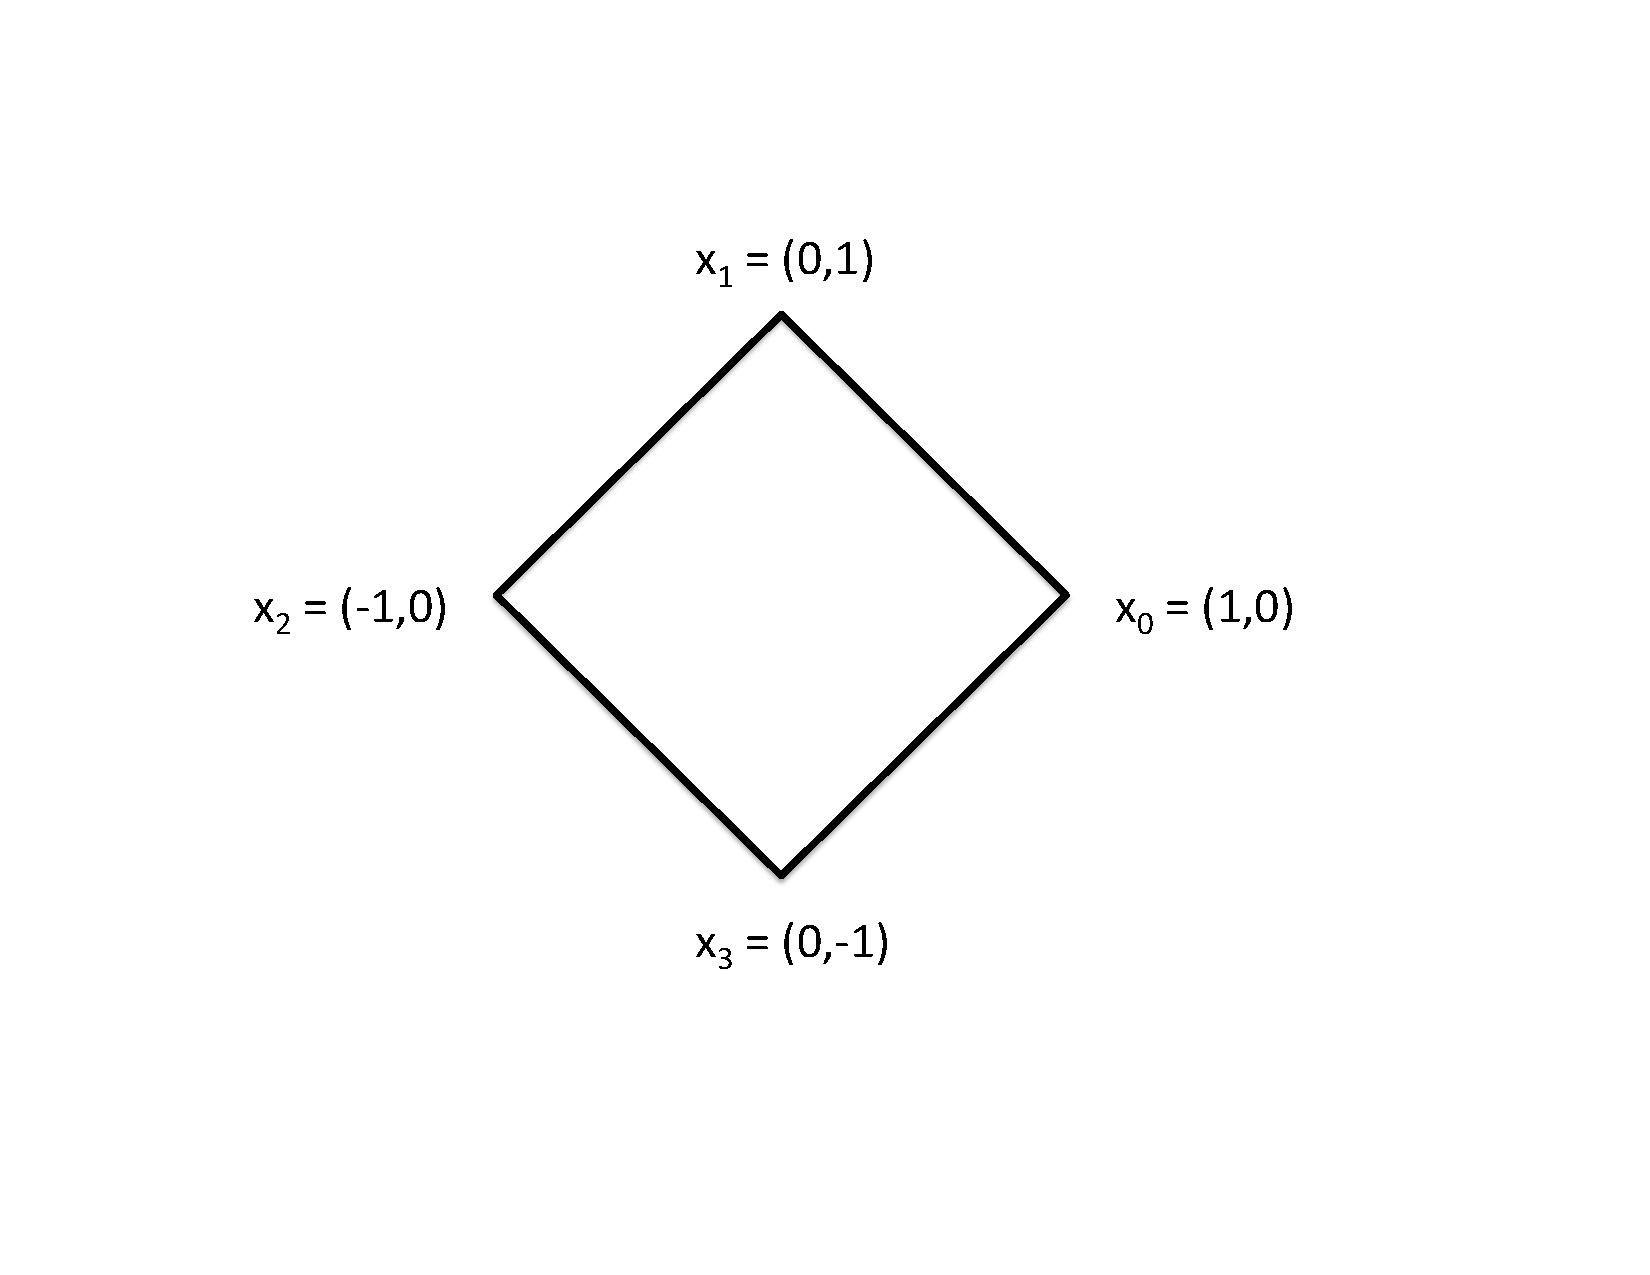
\includegraphics[width=3.0in]{testcase2D.pdf}
	\caption{\small{Four point discretization of the circle.}}\label{fig:testcase2D}
\end{wrapfigure}
Recall that the coefficients in the integrals $I_1,\dotsc,I_4$ are given by
%%%%%%%%%%%%%%%%%%%%%%%%%%%%%%%%%%%%%%%%%%%%%%%%%%%
\baas{
a & = || \bx_{k\pm 1} - \bx_k ||^2 \\
b & =  2(\bx_{k\pm 1} - \bx_k ) \cdot (\bx_j - \bx_{k\pm 1} ) \\
c & = || \bx_j - \bx_{k\pm 1}||^2 + \eps^2.
}
%%%%%%%%%%%%%%%%%%%%%%%%%%%%%%%%%%%%%%%%%%%%%%%%%%%
For the points $\bx_k$ in Fig.~\ref{fig:testcase2D} ($k=0,\dotsc,3$), it is easy to verify that when $\bx_j = \bx_k$, we have
%%%%%%%%%%%%%%%%%%%%%%%%%%%%%%%%%%%%%%%%%%%%%%%%%%%
\baas{
a & = 2, & b & =  -4, & c & = 2 + \eps^2
}
%%%%%%%%%%%%%%%%%%%%%%%%%%%%%%%%%%%%%%%%%%%%%%%%%%%
regardless of the value of $k$ or of whether $k-1$ or $k+1$ is the second point in the coefficients. Since the integrals $I_1,\dotsc,I_4$ depend on $k\pm 1$ only through the coefficients $a,b,c$, the integrals have identical values for $\bx_{k-1}$ and $\bx_{k+1}$. We can then use Eqs.~\eqref{ujkmat} and \eqref{Kk-12D} to see that the 2x2 block relating $\bu(\bx_k)$ to $\ff(\bx_k)$ is given by
%%%%%%%%%%%%%%%%%%%%%%%%%%%%%%%%%%%%%%%%%%%%%%%%%%%
\baas{
\mathcal{K}_{k-1} + \mathcal{K}_{k+1} = \frac{1}{4\pi}\left[2\left(\eps^2 I_2 - I_1\right)\mathcal{I} + \left(\mathcal{A}_{k-1}+\mathcal{A}_{k+1}\right) I_4 + \left(\mathcal{B}_{k-1}+\mathcal{B}_{k+1}\right) I_3 + \left(\mathcal{C}_{k-1}+\mathcal{C}_{k+1}\right) I_2\right].
}
%%%%%%%%%%%%%%%%%%%%%%%%%%%%%%%%%%%%%%%%%%%%%%%%%%%
Using the matrix definitions in Appendix~\ref{app:matentries}, it is easy to verify that for $\bx_j = \bx_k$
%%%%%%%%%%%%%%%%%%%%%%%%%%%%%%%%%%%%%%%%%%%%%%%%%%%
\baas{
\mathcal{A}_{k\pm 1} & = \begin{pmatrix} 1 & \mp 1 \\ \mp 1 & 1 \end{pmatrix}, & \mathcal{C}_{k\pm 1} & = \mathcal{A}_{k\pm 1}, & \mathcal{B}_{k\pm 1} & = -2\mathcal{A}_{k\pm 1},
}
%%%%%%%%%%%%%%%%%%%%%%%%%%%%%%%%%%%%%%%%%%%%%%%%%%%
so that
%%%%%%%%%%%%%%%%%%%%%%%%%%%%%%%%%%%%%%%%%%%%%%%%%%%
\baas{
\mathcal{A}_{k- 1} + \mathcal{A}_{k+1} & = 2\mathcal{I}, & \mathcal{C}_{k- 1} + \mathcal{C}_{k+1} & =  2\mathcal{I}, & \mathcal{B}_{k- 1} + \mathcal{B}_{k+1} & = - 4\mathcal{I},
}
%%%%%%%%%%%%%%%%%%%%%%%%%%%%%%%%%%%%%%%%%%%%%%%%%%%
and 
%%%%%%%%%%%%%%%%%%%%%%%%%%%%%%%%%%%%%%%%%%%%%%%%%%%
\baas{
\mathcal{K}_{k-1} + \mathcal{K}_{k+1} = \frac{1}{2\pi}\left[ - I_1 + (1+\eps^2 )I_2 + -2 I_3 + I_4\right]\mathcal{I}.
}
%%%%%%%%%%%%%%%%%%%%%%%%%%%%%%%%%%%%%%%%%%%%%%%%%%%
So these 2x2 blocks should all be identical diagonal matrices with diagonal values of $(- I_1 + (1+\eps^2 )I_2 + -2 I_3 + I_4)/(2\pi)$.

\end{document}